\chapter{Deployment}
\section{Introduction}
In the following chapter, there will be a walk-through on one of many ways to set up a secure pipeline. The pipeline starts with a source code, which will be explained further, and goes on with pushing the code to GitHub and further to \acrshort{aws}. Within these steps are the security measures and scans discussed previously. Some of these steps are automated using Terraform\footnote{Available at: https://www.terraform.io/} as the programming language. The group has found this repository to be a valuable resource \cite{aws-cicd-pipeline} and used Terraform AWS Documentation\footnote{Available at: https://registry.terraform.io/providers/hashicorp/aws/latest} for information on how to set up the different steps using Terraform. 

\section{Code used in the pipeline}
For testing the group decided on using OWASPs Juice Shop\footnote{Code available at: https://github.com/juice-shop/juice-shop}, which is a deliberately vulnerable web application that is designed to help developers and others learn about web applications security concepts. The code is designed to simulate a real-world application by having common vulnerabilities within the code. The intention is to encourage users to find these vulnerabilities and exploit them and increase the understanding of web application security \cite{owaspJuiceShop}.
The code in the OWASP Juice Shop is open source code on GitHub and is written in TypeScript, which uses a Node.js server and Angular for \gls{front-end} \cite{owaspJuiceShopCode}.
The code contains different vulnerabilities, including SQL injections, cross-site scripting, and many others. 
Overall, OWASP Juice Shop encourages users to improve their skills and it allows for customization and adaption for specific needs from the users. 

\section{Pushing to GitHub}
When the source code is ready to be pushed to GitHub, security measures must be in place. One of the previously mentioned measurements is branch protection. Branch protection rules are easy to enable in GitHub. It is done for each individual repository. GitHub has different rules one can enable, which are explained in \ref{branchprotection}. This can either be done in \gls{GUI} or automated using Terraform, which is shown in Appendix X. 
%\subsection{Access control}
%Something about access control
\begin{comment}
Can easily be enabled in GitHub. Branch protection rules are enables for individual repositories, different repos have different structures and branches. Under settings->Code and automation->Branches you can add branch protection rules. You just enable the ones you want. 
\end{comment}
%\subsection{Signed commits}
\\~\\
Further, the commit signature has to be configured. For signing commits in GitHub, one can either use an SSH or GPG key. These need to be generated and connected to the user's GitHub account. Adding this security measurement increases the authentication of the developer. How to generate and connect a key to a GitHub account is done by following the steps GitHub has provided\footnote{Available at: https://docs.github.com/en/authentication/managing-commit-signature-verification/signing-commits}.

\begin{figure}[H]
    \centering
    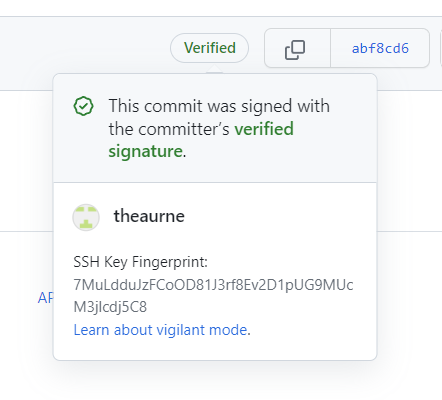
\includegraphics{Images/verified-commit.png}
    \caption{Verified commit in GitHub}
    \label{fig:verified-commit}
\end{figure}

\begin{comment}
Generate a new ssh key:
\begin{tcolorbox}
\begin{verbatim}
$ ssh-keygen -t ed25519 -C "your_email@example.com"
\end{verbatim}
\end{tcolorbox}

You will have to name the file where the public and private key will be saved, let´s call it "example\_key" and assume it was added with the path "\$sim/.ssh"
\\~\\
Add this key to the ssh-agent:\\
\begin{tcolorbox}
\begin{verbatim}
$ ssh-add ~/.ssh/example\_key
\end{verbatim}
\end{tcolorbox}

After this, the key must be added to the GitHub account. Settings->Access->SSH and GPG keys. You add a new SSH key, give it a name, make it a signing key and add the public key.



\begin{figure}[H]
    \centering
    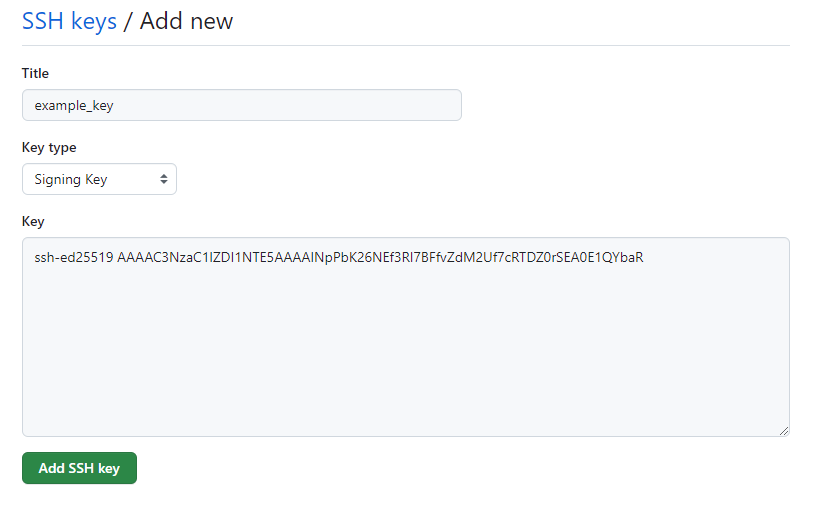
\includegraphics{Images/ssh-key.png}
    \caption{Adding a new SSH key in GitHub}
    \label{fig:ssh_key_github}
\end{figure}

In order to protect your signature from someone who has gotten access to your SSH key, it can be added a passphrase:
\\~\\
\begin{tcolorbox}
\begin{verbatim}
$ ssh-keygen -p -f ~/.ssh/example\_key
\end{verbatim}  
\end{tcolorbox}

Now the key needs to be used for signing. First configure Git to use ssh as key signature:
\begin{tcolorbox}
\begin{verbatim}
$ git config --global gpg.format ssh
\end{verbatim}  
\end{tcolorbox}

Then git needs to know which key you want for signing\\
\begin{tcolorbox}
\begin{verbatim}
$ git config --global user.signingkey ~/.ssh/example_key.pub 
\end{verbatim}
\end{tcolorbox}

Only thing left is signing you commits. This is done by adding the parameter "-S" in your commit:

\begin{tcolorbox}
\begin{verbatim}
$ git commit -S -m "This is a commit
\end{verbatim}
\end{tcolorbox}
When this is done, you have to enter your passphrase, and the commit will be verified.

\begin{figure}[H]
    \centering
    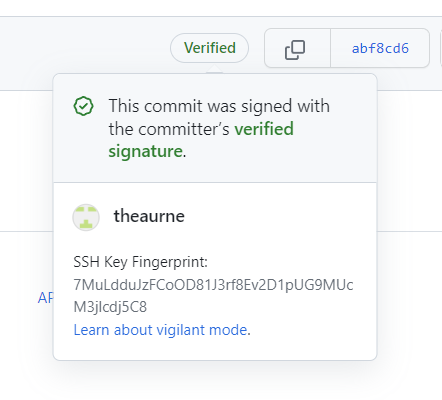
\includegraphics{Images/verified-commit.png}
    \caption{Verified commit in GitHub}
    \label{fig:verified-commit}
\end{figure}
\end{comment}

\section{Managing security in GitHub}
After the source code is pushed to its belonging branch, the code must be scanned for potential vulnerabilities before moving forward. One of these scans is SAST scanning using CodeQL. Setting up CodeQL\footnote{Intructions available at: https://docs.github.com/en/code-security/code-scanning/automatically-scanning-your-code-for-vulnerabilities-and-errors/configuring-code-scanning-for-a-repository} is done by adding the CodeQL YAML file in the workflow. Other security tools in GitHub are Dependabot\footnote{Instructions available at: https://docs.github.com/en/code-security/dependabot/dependabot-security-updates/configuring-dependabot-security-updates} and Secret scanner\footnote{Instructions available at: https://docs.github.com/en/code-security/secret-scanning/configuring-secret-scanning-for-your-repositories}. These are also enabled in the security settings. After being enabled, all these tools automatically scan the code for vulnerabilities. 

\section{Committing the source code to AWS}
When all vulnerabilities are detected and fixed in GitHub, the source code can be built in \acrshort{aws}. In order for this to be done, a connection between the \acrshort{aws} and GitHub account needs to be made. AWS CodeStar Connection enables the connection of cloud resources to external code repositories, such as the Juice-Shop repository on GitHub. By creating this connection as a resource, it can be used by AWS CodePipeline to automatically trigger the pipeline in response to any changes made to the GitHub repository.
This can either be done on the \acrshort{aws} website or by using Terraform to create a connection resource with GitHub as the provider. 

\begin{tcolorbox}
\begin{verbatim}
resource "aws_codestarconnections_connection" "code-connection" {
  name          = "code-connection"
  provider_type = "GitHub"
}    
\end{verbatim}
\end{tcolorbox}

Following the successful creation of the connection resource in \acrshort{aws} using Terraform, a manual verification process in AWS is required. This is essential due to the requirement to log in to the system with one's GitHub account credentials, as passing secrets through AWS to GitHub login is not possible, due to the connection opening a third-party login page that AWS does not control.

\section{Storing artifacts}
To store \gls{artifact}s generated during different stages of the pipeline, an S3 bucket is created. The bucket is created as a resource with optional 

One crucial aspect to consider is the need for unique bucket names within the server area, as \acrshort{aws} uses this as a means to differentiate between buckets owned by different users.

\begin{tcolorbox}
\begin{verbatim}
resource "aws_s3_bucket" "codepipeline_artifact" {
  bucket = "artifact-bucket-unique-name"
}
\end{verbatim}
\end{tcolorbox}

In order for each stage to be able to access the S3 bucket and retrieve the last stage's \gls{artifact}s, it has to be given access to the bucket. These access rights have to be individually given to each stage in the pipeline. In the following code the pipeline and every stage is given access to the bucket, hence the "s3:*".

\begin{tcolorbox}
\begin{verbatim}
statement {
    sid       = ""
    actions   = ["s3:*", "codebuild:*"]
    resources = ["*"]
    effect    = "Allow"
}
\end{verbatim}
\end{tcolorbox}

\begin{comment}
\begin{tcolorbox}
\begin{verbatim}
data "aws_iam_policy_document" "tf-cicd-build-policies" {
    statement {
        sid       = ""
        actions   = ["logs:*", "s3:*", "codebuild:*", "secretsmanager:*", 
        "iam:*"]
        resources = ["*"]
        effect    = "Allow"
  }
}
\end{verbatim}
\end{tcolorbox}
\end{comment}

\section{The build stage}
The build stage has three key components: the build resource, the \gls{buildspec} file, and the \acrshort{iam}. Then link the build resource to the pipeline resource. The key point in the build resource is the container you are building an environment where we set up a temporary container from AWS's pre-built images. The key point in building resources is the container being built as an environment where a temporary container is set up using pre-built images from AWS. 


\begin{tcolorbox}
\begin{verbatim}  
environment {
    compute_type                = "BUILD_GENERAL1_SMALL"
    image                       = "aws/codebuild/standard:6.0"
    type                        = "LINUX_CONTAINER"
    image_pull_credentials_type = "CODEBUILD"
}
source {
    type      = "CODEPIPELINE"
    buildspec = file("buildspec/buildspec.yml")
}
\end{verbatim}
\end{tcolorbox}

The advantage of this is that it makes it easier for us to set up the dependencies needed when building the code. Because through the \gls{buildspec} file, we can easily specify that it should come with the prerequisites we need to run a test build. The important thing here is that we specify that we are doing a build test and not a full build for code deployment, since the code will keep running as if the container is set up but will never complete if we do a full build.
\begin{tcolorbox}
\begin{verbatim}
version: 0.2

phases:
  install:
    runtime-versions:
      nodejs: latest
  pre_build:
    commands:
      - npm install
      - npm update
  build:
    commands:
       - npm run test:server
\end{verbatim}
\end{tcolorbox}

To integrate the installation of node so we can build and run the code with the rest of the pipeline and permissions to S3 as mentioned earlier, we use \acrshort{iam} roles from before and connecting to the build resource.

\begin{tcolorbox}
\begin{verbatim}
service_role = aws_iam_role.tf-codebuild-role.arn
\end{verbatim}
\end{tcolorbox}


\subsection{Signed Artifacts}


\subsection{OWASP Zap}


\subsection{Penetration testing}



